\chapter{Methodik}
\label{chap:methodology}

\section{Abkürzungen}

Man kann Abkürzungen definieren und wie folgt darauf verweisen: Die \gls{dsr}-Methodik wird häufig in der Forschung zu Informationssystemen verwendet. Der \gls{dsr}-Ansatz betont die Erstellung und Evaluierung von Artefakten zur Lösung identifizierter Probleme.

\section{Abbildungen}

\begin{figure}[htbp!]
    \centering
    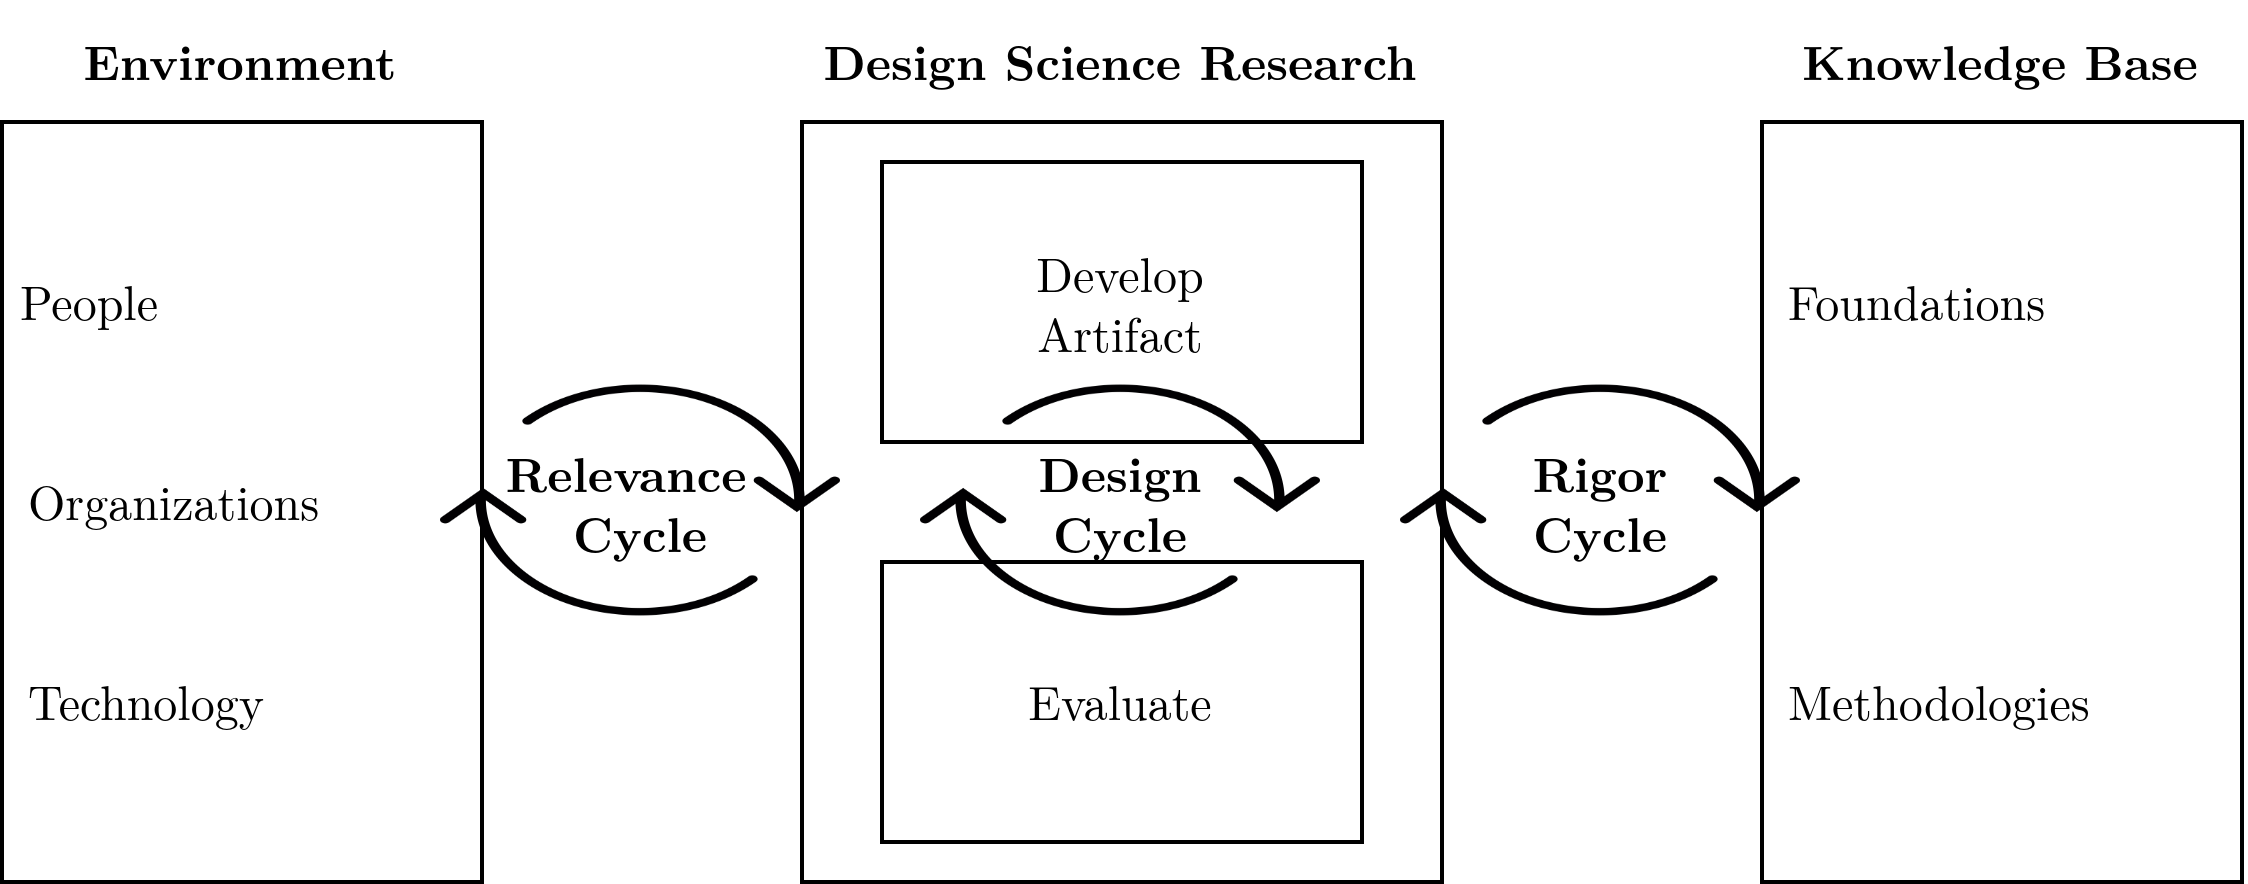
\includegraphics[width=0.9\textwidth]{figures/design-science-generic.png}
    \caption[DSR-Ansatz mit Relevanz-, Rigorositäts- und Design-Zyklus.]{DSR-Ansatz mit Relevanz-, Rigorositäts- und Design-Zyklus. Adaptiert aus~\textcite{hevner2004design}.}
    \label{fig:design-science-generic}
\end{figure}

Man kann Abbildungen einfügen und wie folgt darauf verweisen: Abbildung~\ref{fig:design-science-generic} zeigt den \gls{dsr}-Ansatz mit Relevanz-, Rigorositäts- und Design-Zyklus.
